\documentclass[12pt, a4paper, simple]{eskdtext}

\usepackage{hyperref}
\usepackage{_env/gpi_global.env}
\usepackage{_env/gpi_report.env}
\usepackage{_sty/gpi_lst}
\usepackage{_sty/gpi_toc}
\usepackage{_sty/gpi_t}
\usepackage{_sty/gpi_p}
\usepackage{_sty/gpi_u}

% Код
% \ESKDletter{О}{Л}{Р}
% \def \gpiDocTypeNum {81}
% \def \gpiDocVer {00}
% \def \gpiCode {\ESKDtheLetterI\ESKDtheLetterII\ESKDtheLetterIII.\gpiStudentGroupName\gpiStudentGroupNum.\gpiStudentCard-0\gpiDocNum~\gpiDocTypeNum~\gpiDocVer}

\def \gpiDocTopic {Отчёт лабораторной работы №\gpiDocNum}

% Графа 1 (наименование изделия/документа)
% \ESKDcolumnI {\ESKDfontII \gpiTopic \\ \gpiDocTopic}

% Графа 2 (обозначение документа)
% \ESKDsignature {\gpiCode}

% Графа 9 (наименование или различительный индекс предприятия) задает команда
% \ESKDcolumnIX {\gpiDepartment}

% Графа 11 (фамилии лиц, подписывающих документ) задают команды
% \ESKDcolumnXIfI {\gpiStudentSurname}
% \ESKDcolumnXIfII {\gpiTeacherSurname}
% \ESKDcolumnXIfV {\gpiTeacherSurname}

\begin{document}
    \begin{ESKDtitlePage}
    \ESKDstyle{empty}
    \begin{center}
        \gpiMinEdu \\
        \gpiEdu \\
        \gpiKaf \\
    \end{center}

    \vfill

    \begin{center}
        \gpiTopic
    \end{center}

    \vfill

    \begin{center}
        \textbf{\gpiDocTopic} \\
        ПО ДИСЦИПЛИНЕ \gpiDiscipline \\
    \end{center}

    \vfill

    \begin{flushright}
        \begin{minipage}[t]{7cm}
            Выполнил:\\
            \PageTitleStudentInfo
            \PageTitleDateField
            \hspace{0pt}

            Проверил:\\
            \PageTitleTeacherInfo
            \PageTitleDateField
        \end{minipage}
    \end{flushright}

    \vfill

    \begin{center}
        \PageTitleCity~\ESKDtheYear
    \end{center}
\end{ESKDtitlePage}

    \ESKDstyle{empty}
    \begin{center}
        \textbf{\gpiDocTopic}
    \end{center}

    % = = = = = = = =
    \paragraph{} \textbf{Тема}: <<\gpiTopicRep>>

    \paragraph{} \textbf{Цель}: Разработка многооконного приложения,
    предоставляющего возможности: воспроизведения аудио и видео файлов,
    создания фотоснимков.

    \paragraph{} \textbf{Что нужно сделать}:

    Разработать многооконное приложения, включающая в себя слудующие активности:
    активность создания фотоснимка,
    активность прослушивания аудио,
    активность просмотра видео,
    активность пролистывания картинок.

    \paragraph{} \textbf{Разработка дизайна}:

    \begin{figure}[!h]
        \centering
        \begin{minipage}{0.19\textwidth}
            \centering
            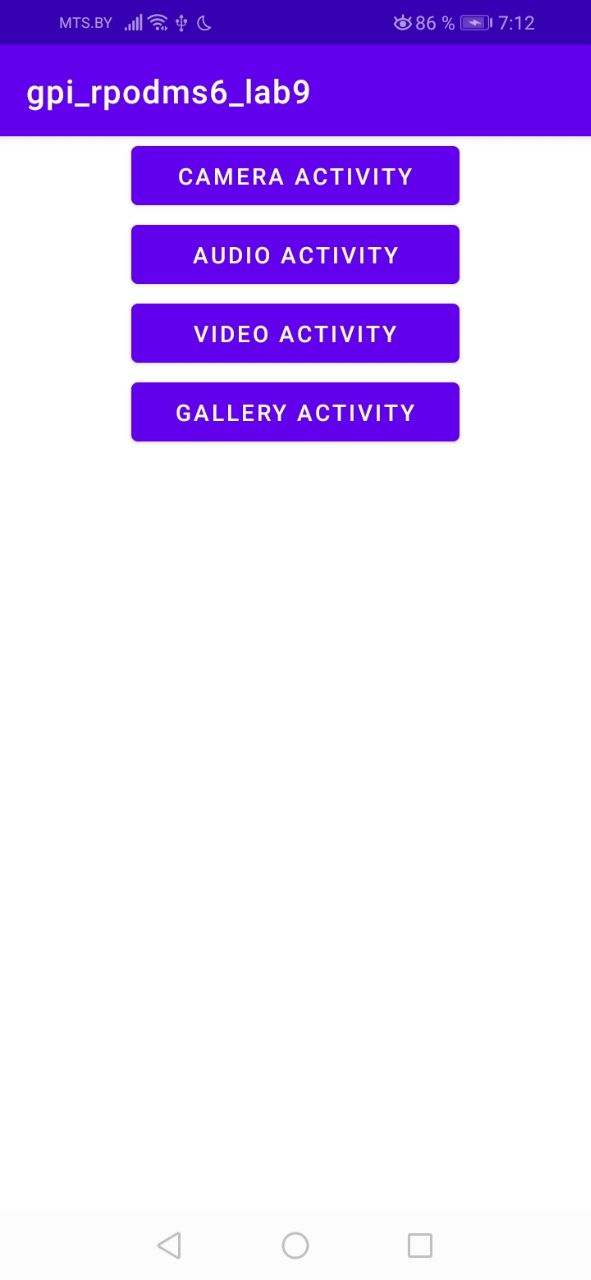
\includegraphics[width=\linewidth]
                {_assets/MainActivity.jpg}
            \caption{MainActivity}
        \end{minipage}
        \begin{minipage}{0.19\textwidth}
            \centering
            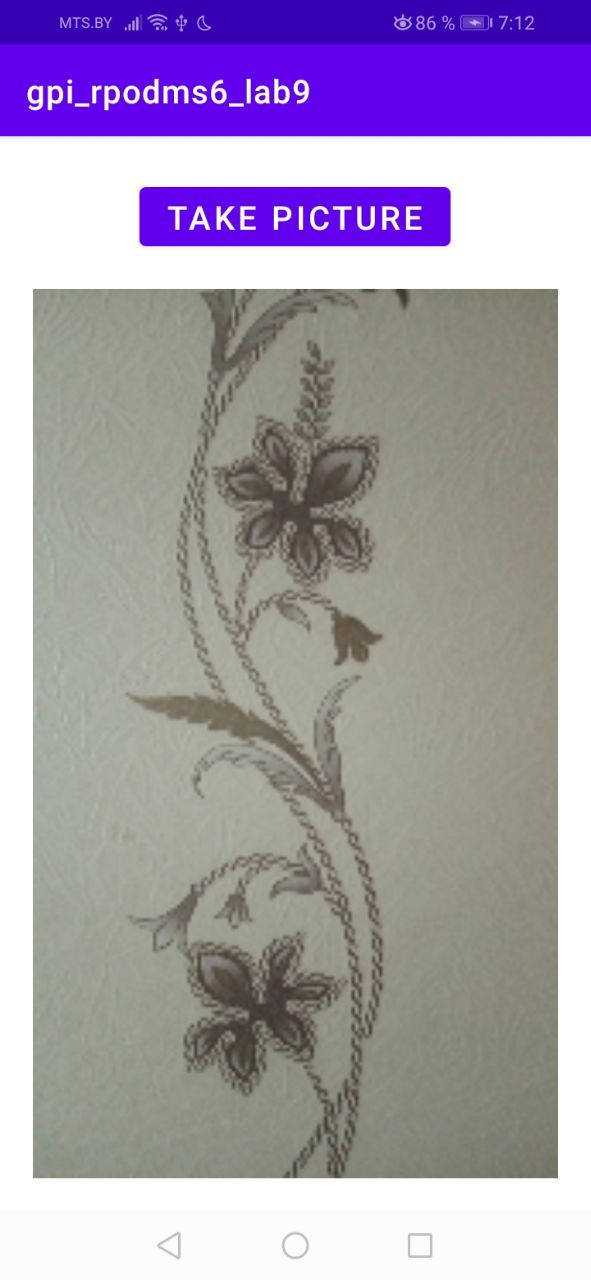
\includegraphics[width=\linewidth]
                {_assets/CameraActivity.jpg}
            \caption{CameraActivity}
        \end{minipage}
        \begin{minipage}{0.19\textwidth}
            \centering
            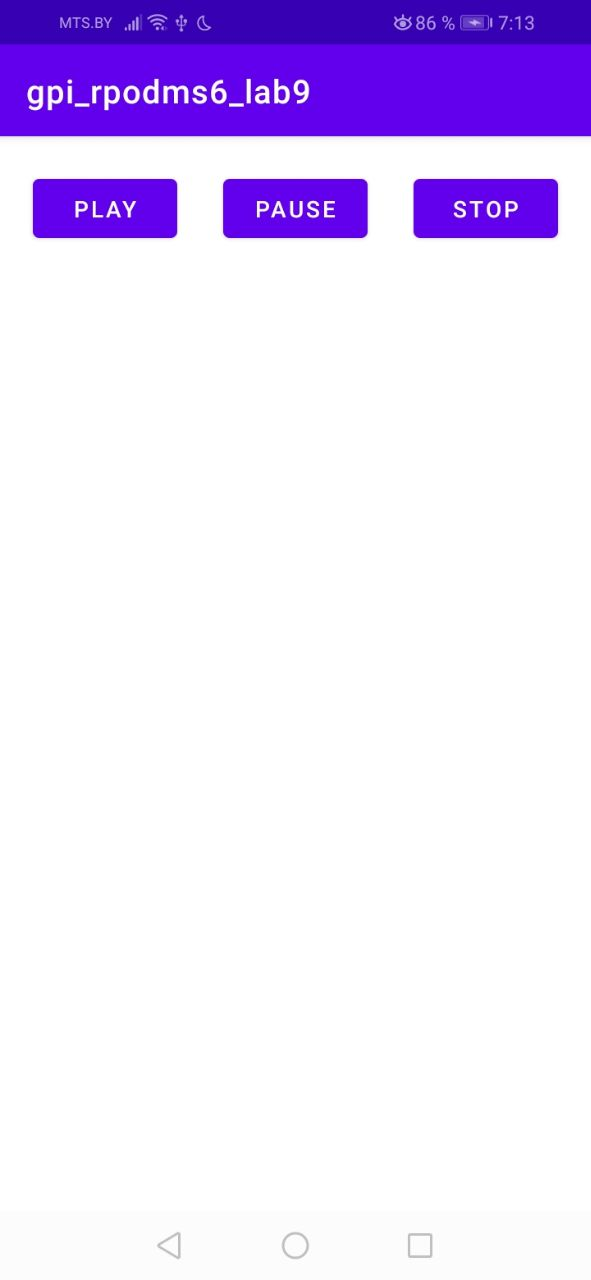
\includegraphics[width=\linewidth]
                {_assets/AudioActivity.jpg}
            \caption{AudioActivity}
        \end{minipage}
        \begin{minipage}{0.19\textwidth}
            \centering
            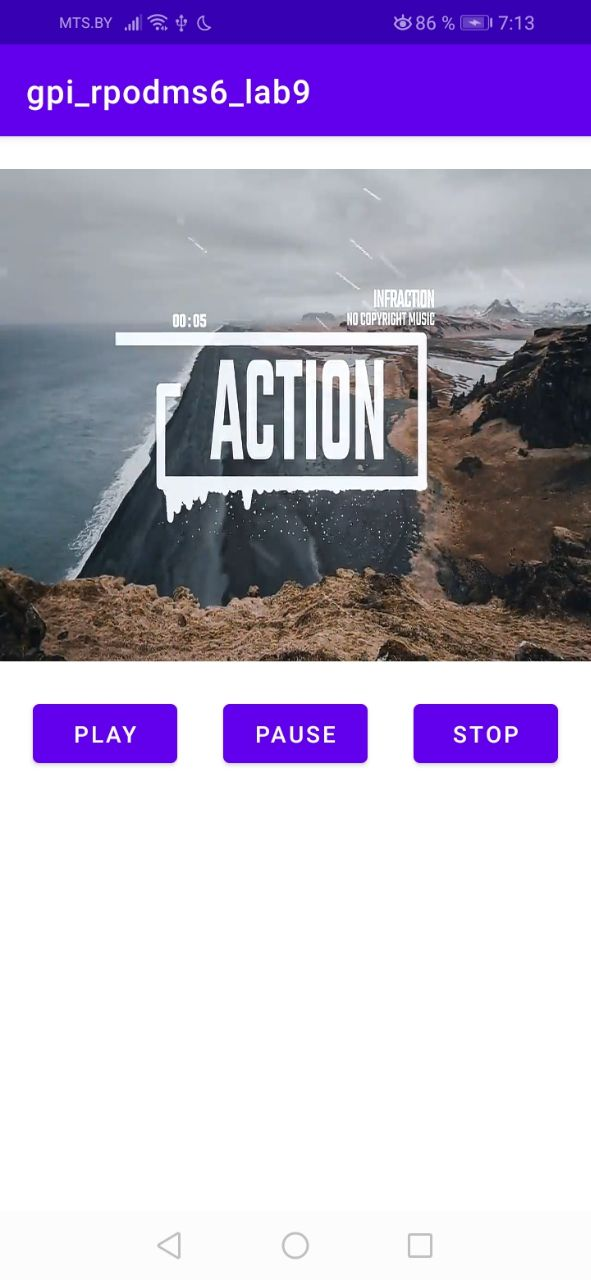
\includegraphics[width=\linewidth]
                {_assets/VideoActivity.jpg}
            \caption{VideoActivity}
        \end{minipage}
        \begin{minipage}{0.19\textwidth}
            \centering
            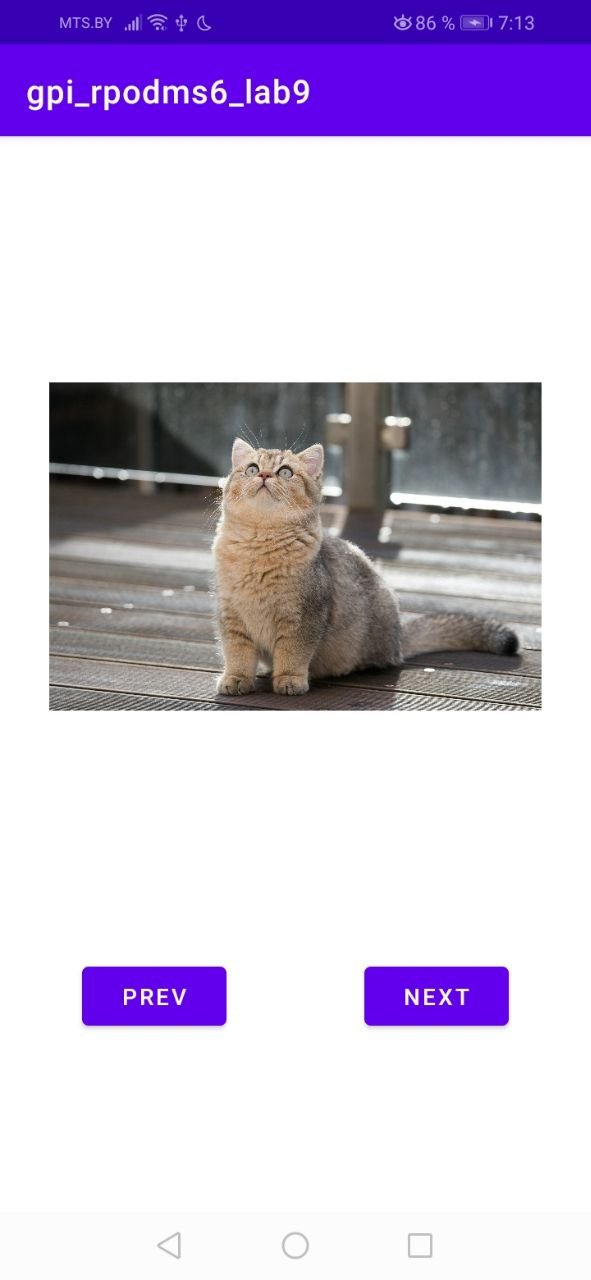
\includegraphics[width=\linewidth]
                {_assets/GalleryActivity.jpg}
            \caption{GalleryActivity}
        \end{minipage}
    \end{figure}

    \paragraph{} \textbf{Исходный код}: 
    
    \lstinputlisting[language=xml, name=app/src/main/res/values/strings.xml]
    {../sources/app/src/main/res/values/strings.xml}

    \lstinputlisting[language=xml, name=app/src/main/AndroidManifest.xml]
    {../sources/app/src/main/AndroidManifest.xml}

    \begin{figure}[!h]
        \centering
        \begin{minipage}{0.19\textwidth}
            \centering
            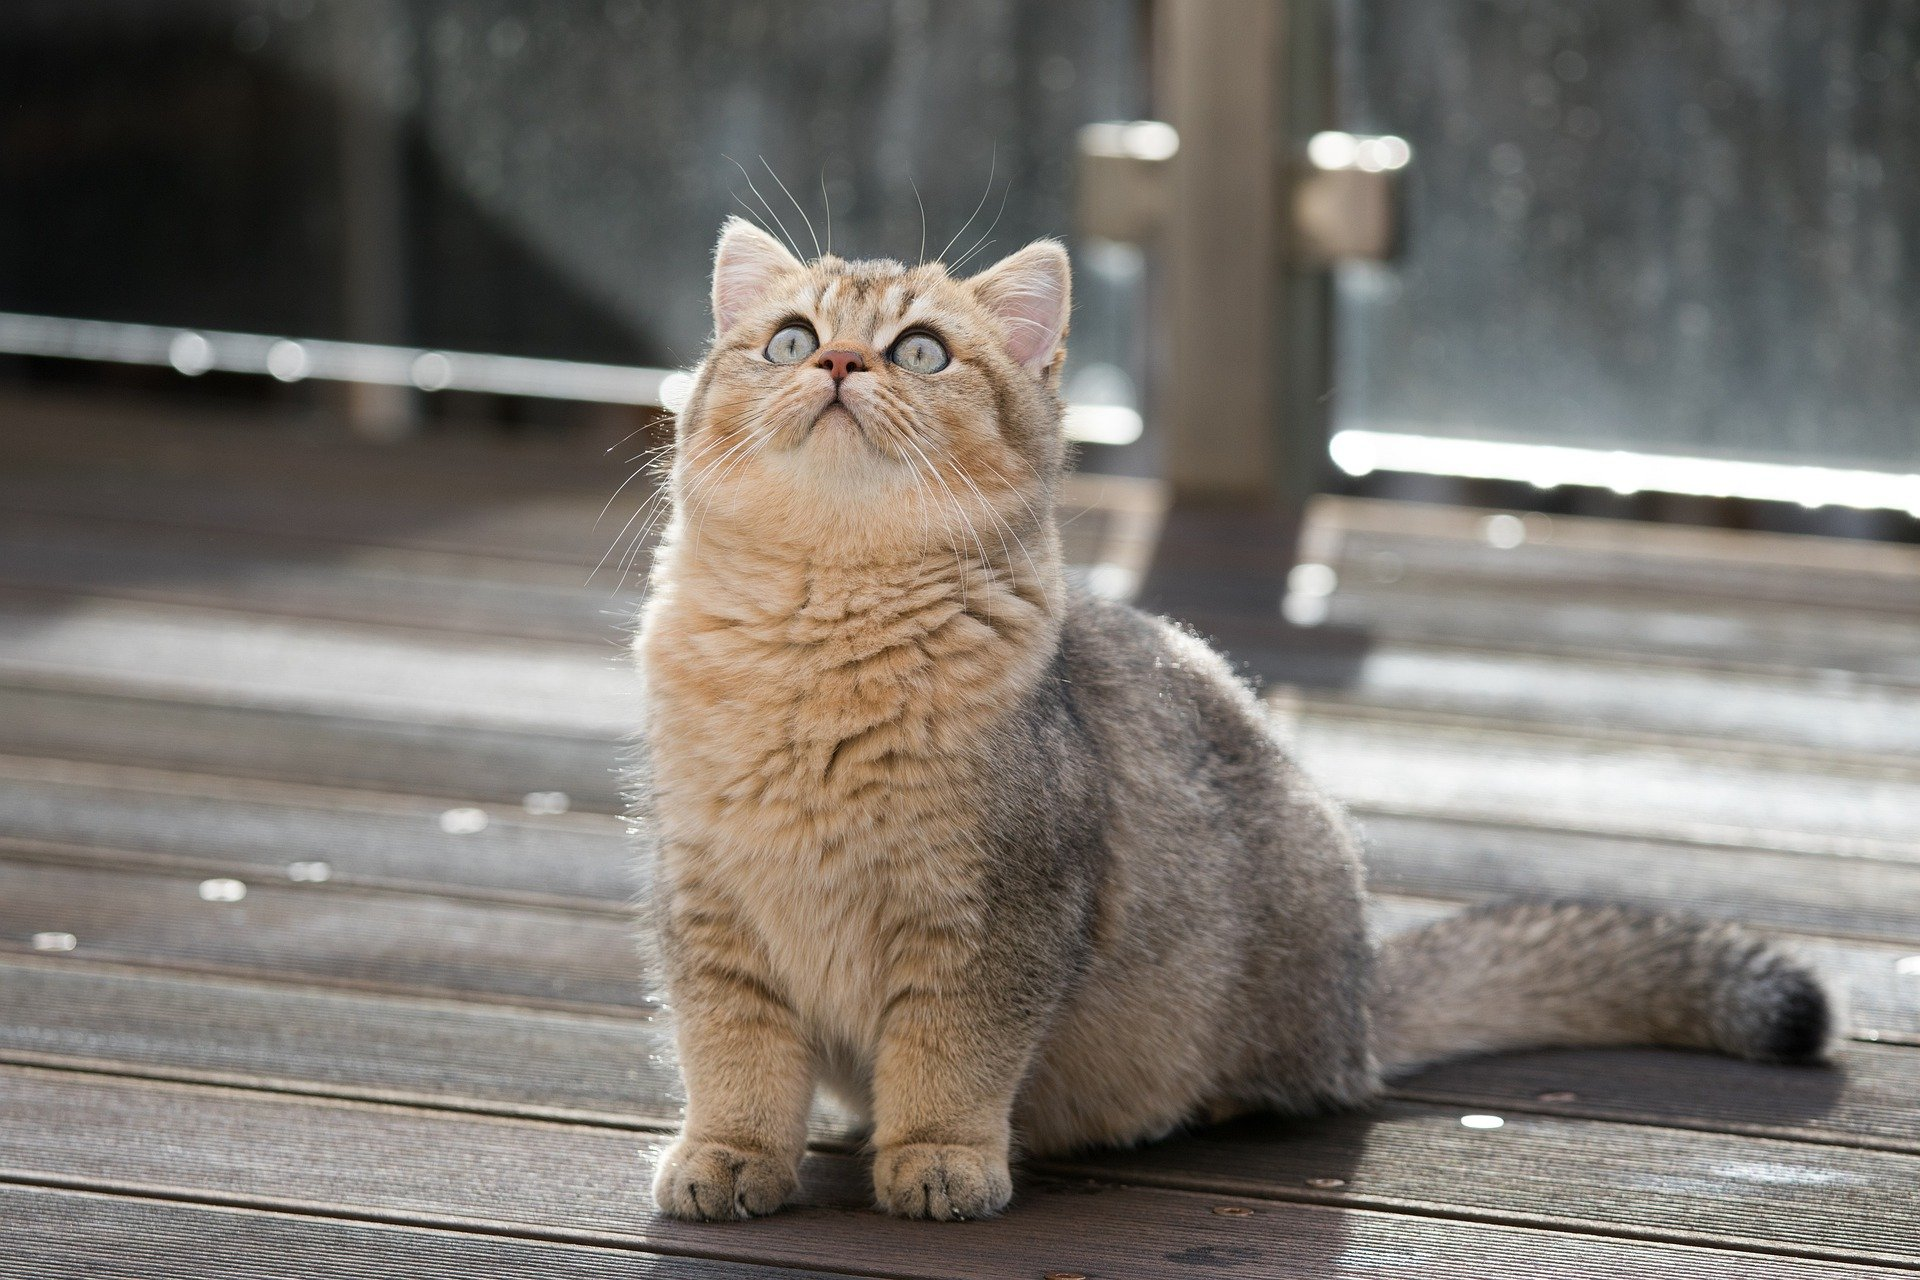
\includegraphics[width=\linewidth]
                {../sources/app/src/main/res/drawable/picture1.jpg}
            \caption{Картинка 1}
        \end{minipage}
        \begin{minipage}{0.19\textwidth}
            \centering
            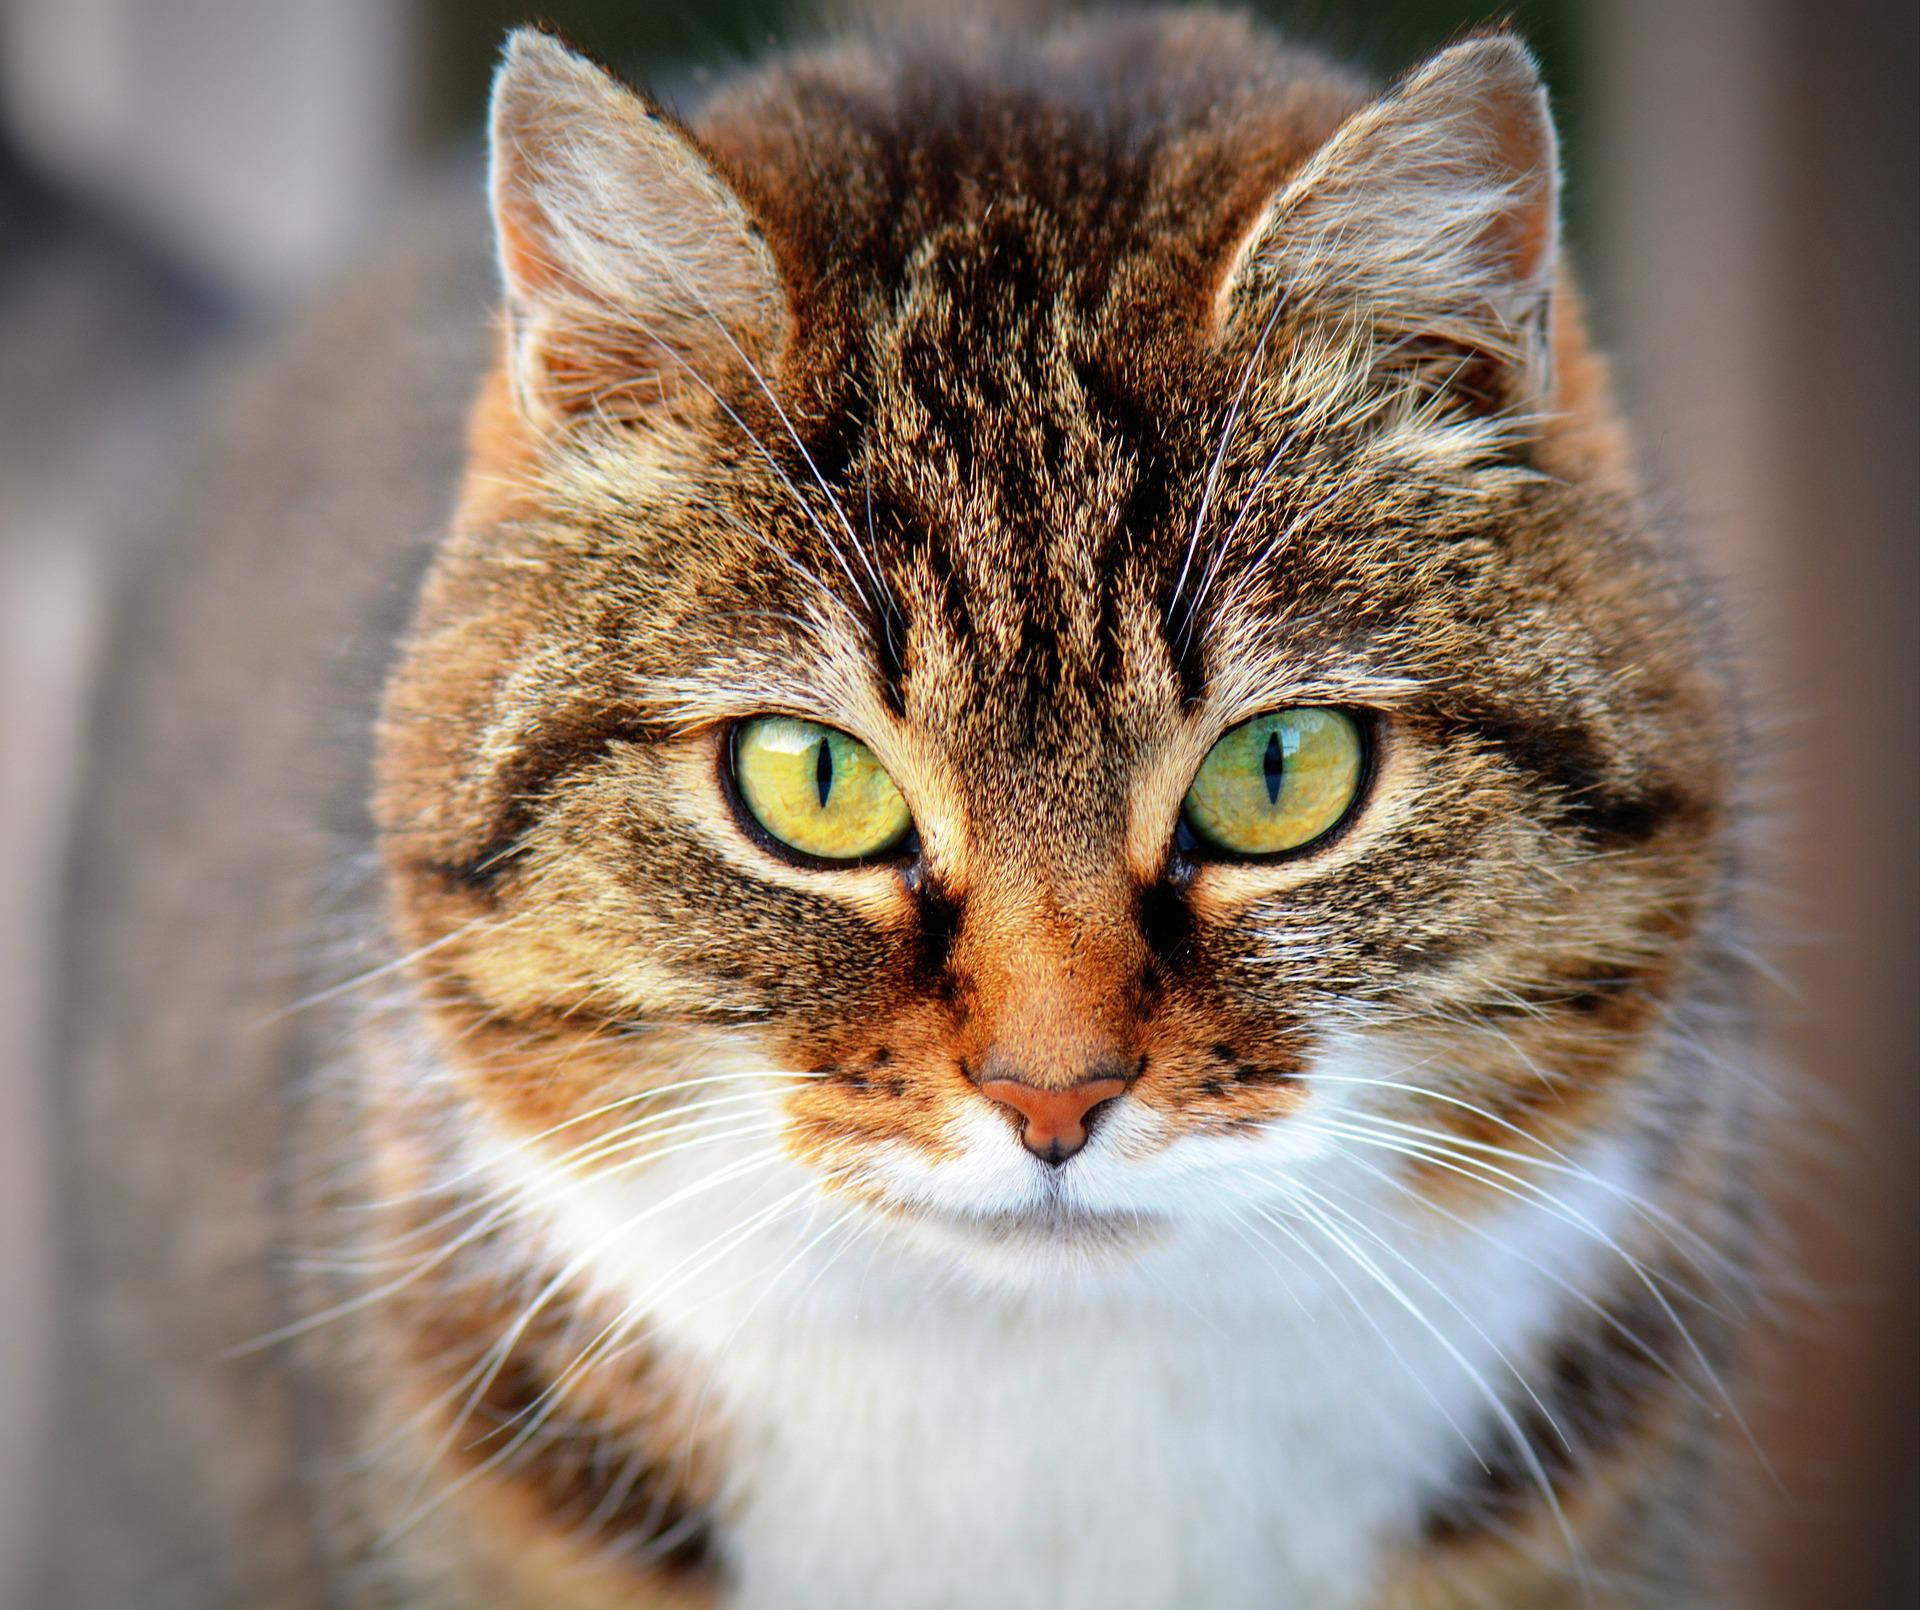
\includegraphics[width=\linewidth]
                {../sources/app/src/main/res/drawable/picture2.jpg}
            \caption{Картинка 2}
        \end{minipage}
        \begin{minipage}{0.19\textwidth}
            \centering
            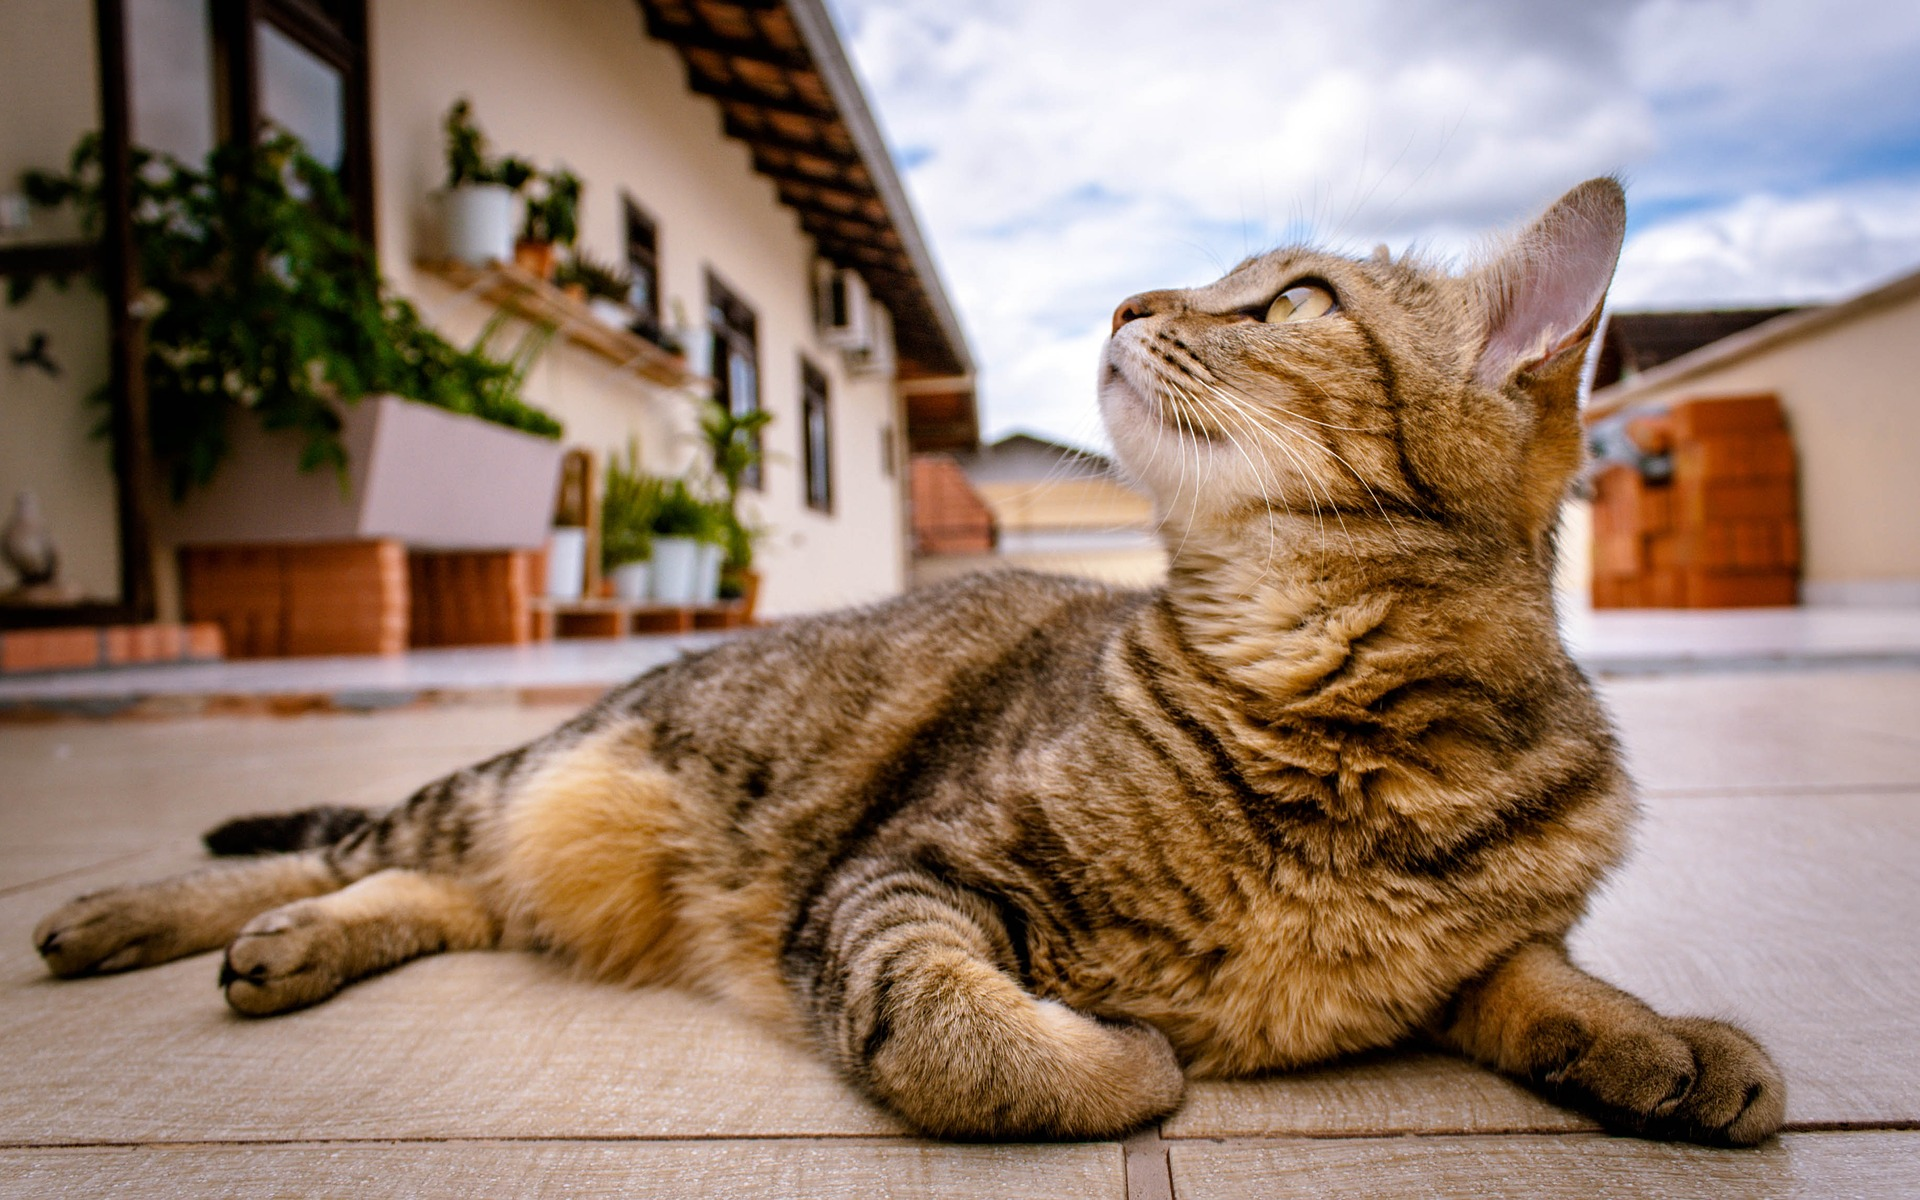
\includegraphics[width=\linewidth]
                {../sources/app/src/main/res/drawable/picture3.jpg}
            \caption{Картинка 3}
        \end{minipage}
        \begin{minipage}{0.19\textwidth}
            \centering
            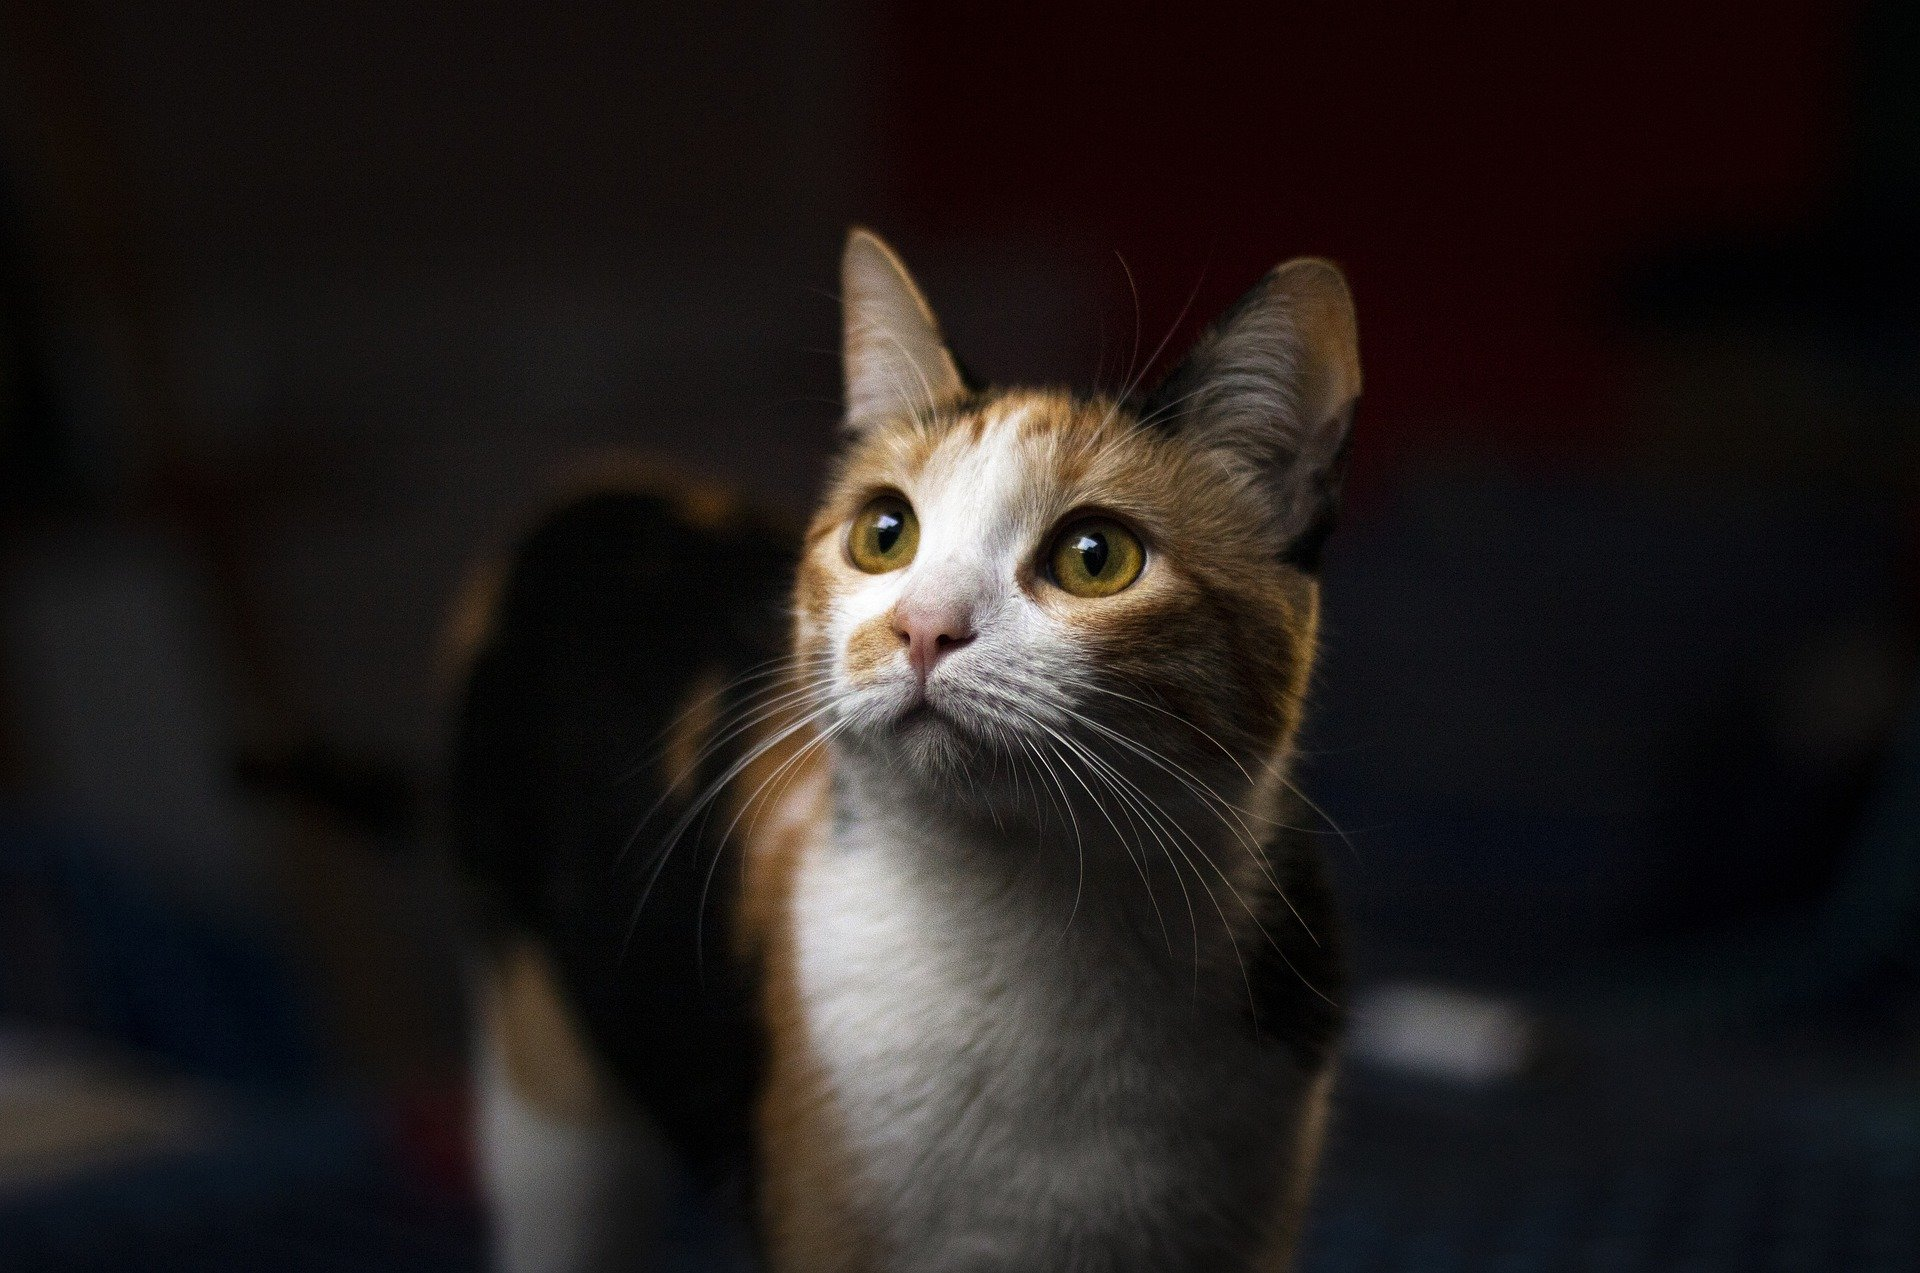
\includegraphics[width=\linewidth]
                {../sources/app/src/main/res/drawable/picture4.jpg}
            \caption{Картинка 4}
        \end{minipage}
        \begin{minipage}{0.19\textwidth}
            \centering
            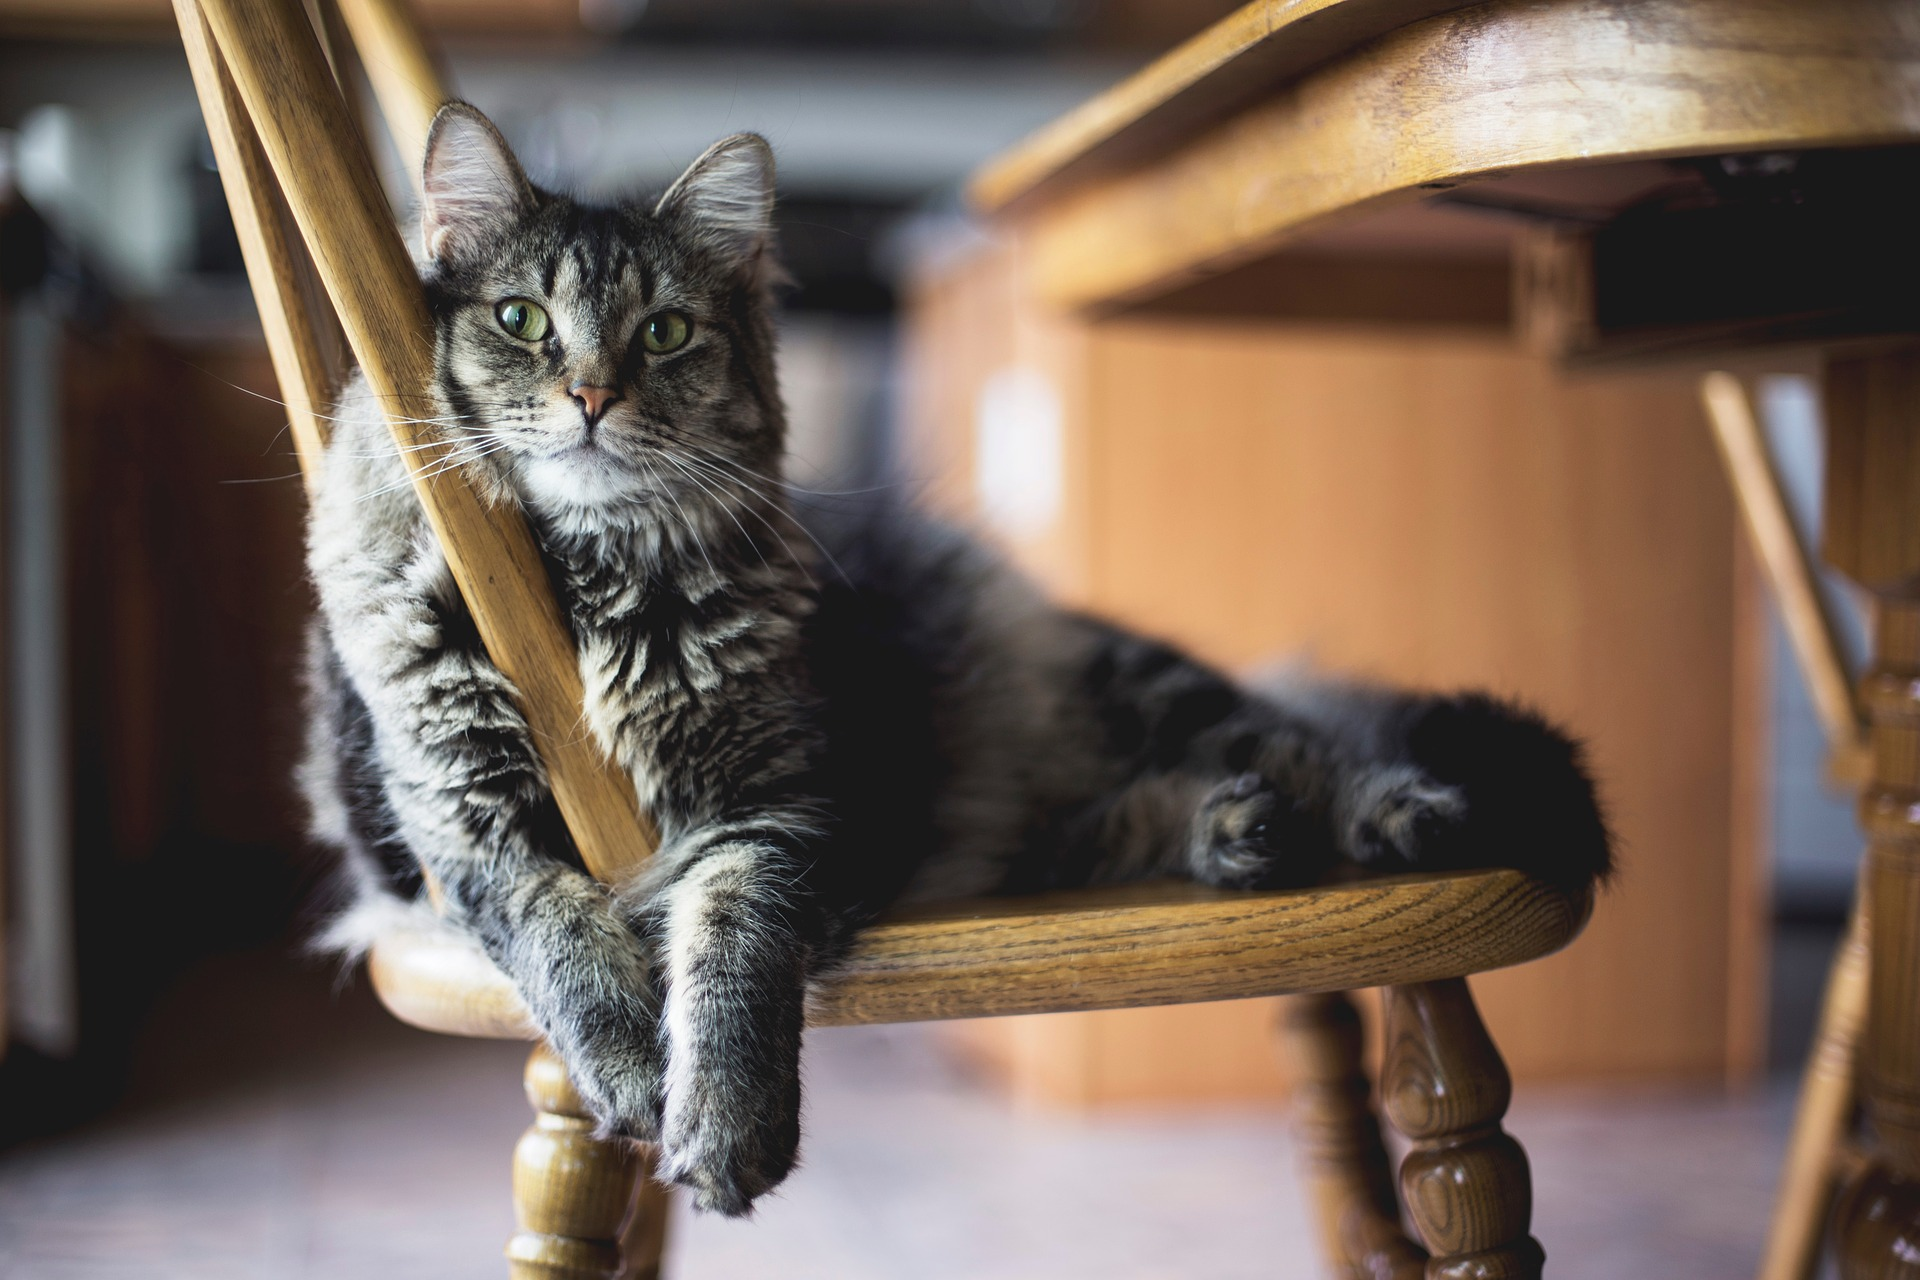
\includegraphics[width=\linewidth]
                {../sources/app/src/main/res/drawable/picture5.jpg}
            \caption{Картинка 5}
        \end{minipage}
    \end{figure}


    \lstinputlisting[language=xml, name=app/src/main/res/layout/activity_main.xml]
    {../sources/app/src/main/res/layout/activity_main.xml}

    \lstinputlisting[language=java, name=app/src/main/java/.../MainActivity.java]
    {../sources/app/src/main/java/com/example/gpi_rpodms6_lab9/MainActivity.java}

    
    \lstinputlisting[language=xml, name=app/src/main/res/layout/activity_camera.xml]
    {../sources/app/src/main/res/layout/activity_camera.xml}

    \lstinputlisting[language=java, name=app/src/main/java/.../CameraActivity.java]
    {../sources/app/src/main/java/com/example/gpi_rpodms6_lab9/CameraActivity.java}


    \lstinputlisting[language=xml, name=app/src/main/res/layout/activity_audio.xml]
    {../sources/app/src/main/res/layout/activity_audio.xml}

    \lstinputlisting[language=java, name=app/src/main/java/.../AudioActivity.java]
    {../sources/app/src/main/java/com/example/gpi_rpodms6_lab9/AudioActivity.java}


    \lstinputlisting[language=xml, name=app/src/main/res/layout/activity_video.xml]
    {../sources/app/src/main/res/layout/activity_video.xml}

    \lstinputlisting[language=java, name=app/src/main/java/.../VideoActivity.java]
    {../sources/app/src/main/java/com/example/gpi_rpodms6_lab9/VideoActivity.java}


    \lstinputlisting[language=xml, name=app/src/main/res/layout/activity_gallery.xml]
    {../sources/app/src/main/res/layout/activity_gallery.xml}

    \lstinputlisting[language=java, name=app/src/main/java/.../GalleryActivity.java]
    {../sources/app/src/main/java/com/example/gpi_rpodms6_lab9/GalleryActivity.java}

%     \begin{lstlisting}[caption=Вывод в консоль]
%  Hello, World!
% \end{lstlisting}

    \paragraph{} \textbf{Вывод}:
    Создали активность для фотоснимков с камеры.
    Создали активность прослушивания аудио.
    Создали активность просмотра видео.
    Создали активность пролистывания картинок.

    % = = = = = = = =
    % \newpage
    % \addcontentsline{toc}{section}{Список использованных источников}
    \section*{Список использованных источников}
    \begin{enumerate}
        \item[1.] Кондратюк, А.П. Разработка приложений для мобильных операционных систем «Android» :
        ЭУМК для студ. второй ступени (магистратуры) специальности 1-31 81 06 <<Веб-программирование и интернет-технологии>>
        физ.-мат. фак. / А.П. Кондратюк ; Брест. гос. ун-т им. А.С. Пушкина, каф. ПМиИ. – Брест :
        электрон. издание БрГУ, 2016. – 469 с.\\
        §21. Лабораторная работа №7, cc. 415-452
        % \item[1.] eskdx.pdf [Электронный ресурс]
        % - Режим доступа: \url{http://tug.ctan.org/macros/latex/contrib/eskdx/manual/eskdx.pdf}.
        % Дата~доступа:~20.02.2022.
    \end{enumerate}
    \newpage
\end{document}
